\documentclass{article}
\usepackage{graphicx} % Required for inserting images
\usepackage[a4paper, margin=1.2in]{geometry}
\usepackage{amsmath}
\usepackage{amssymb}

\usepackage{hyperref}

\title{Exploring Aliasing and the Sampling Theorem} %\\\large\textit{Approximation Part 2 Assignment}}
\author{Margherita Tonon}
\date{April 2025}

\begin{document}

\maketitle

\section{Introduction}
%introduction sentence, context, motivation

\section{Background}
In signal processing, two types of signals exist: analog signals and digital signals. %check that this is true/rephrase
An analog signal refers to a signal that varies continuously over time. 
The complexity of analog signal processing, their susceptibility to noise and signal degradation over time, as well as their limited reproductibility and scalability makes them inconvenient to work with in practice. 
Therefore, digital signals are used -- signals that vary discretely over time and can take only a finite number of distinct values.
%mention advantages of digital signals?

Sampling refers to the process of converting an analog signal into a digital signal. If we let $x(t)$ be a continuous time signal, the sampled signal $x[n]$ is defined as
\begin{center}
    \begin{math}
        x[n] = x(nT_s)
    \end{math}  
\end{center}
where $n$ represents discrete time sampling points and $T_s$ represents the sampling period, such that the sampling frequency $f_s = \frac{1}{T_s}$.

Sampling can also be represented as 
\begin{center}
    \begin{math}
        x_s(t) = x(t) \sum_{-\infty}^{\infty} \delta (t-nT_s)
    \end{math}  
\end{center}
where $x_s(t)$ is the sampled points, and $\delta$ is the dirac delta distribution, taking value 1 if $t=nT_s$ and 0 otherwise.
Therefore, it is clear that when $t=nT_s$, $x_s(t) = x(t)$; otherwise, $x_s(t) = 0$. 

In practice, sampling allows us to discretize a continuous input, facilitating the handling of signals. After sampling is done, it is natural that the signal must be reconstructed in order to recover the original (time continuous) signal.
However, recovery is not always perfect -- the Shannon-Nyquist condition must be met.
%something along the lines of: the key issue is what must the sampling frequency be in order for a signal to be perfectly reconstructed and recovered?

The Shannon-Nyquist theorem states that a signal can be perfectly reconstructed if the sampling frequency is greater than two times the maximum frequency $B$ of the continuous signal:
\begin{center}
    \begin{math}
        f_s > 2B
    \end{math}  
\end{center}
For example, if we consider a sine wave with frequency 5 Hertz, $\sin(2\pi \cdot 5 \cdot t)$, once sampled it can be perfectly reconstructed if the sampling frequency is greater than 10.
%TODO: need to check what the relationship between B and the max continuous frequency is

%do i explain quantization here?

In the time domain, a sampled signal looks like discrete spikes (Figure 1). 
\begin{figure}
    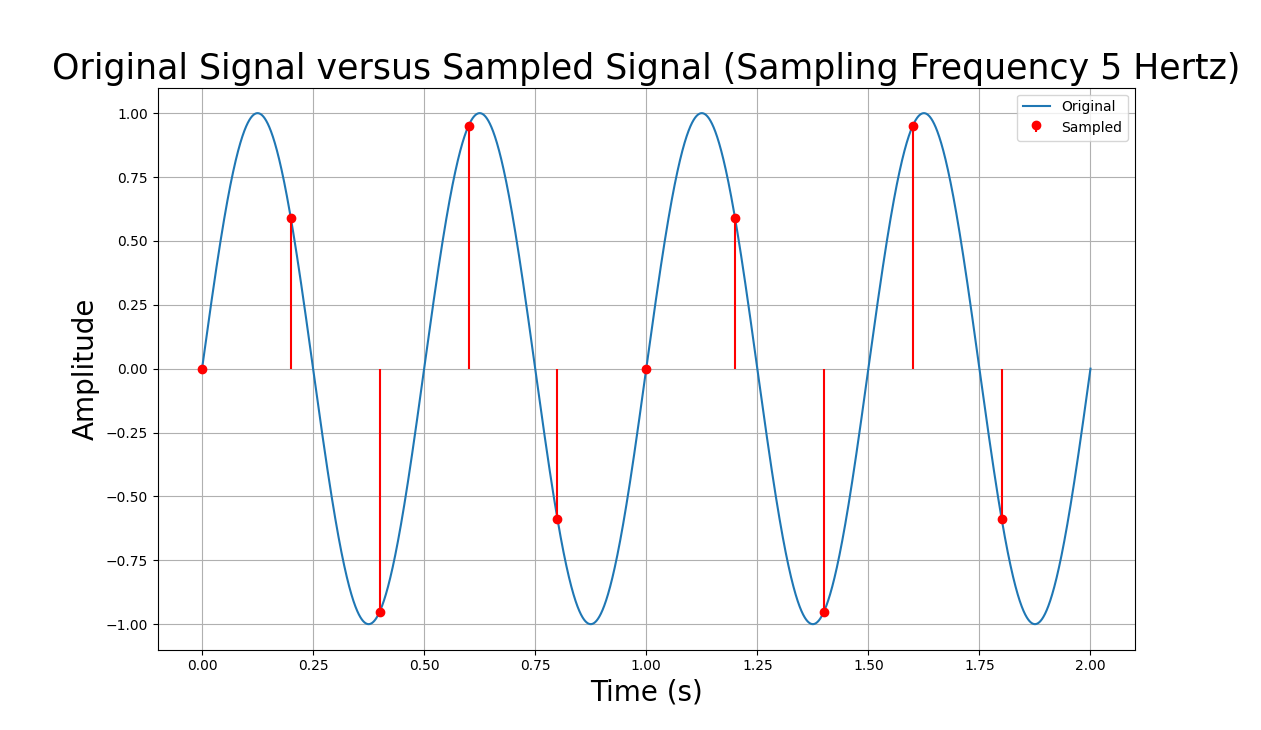
\includegraphics[width=\linewidth]{ogvssampled_BIG.png}
    \caption{Representation of sampling of $\sin(4\pi t)$ in the time domain, sampled at a frequency of 5 Hertz}
    \label{fig:grid}

\end{figure}
The Fourier Transform allows us to transition from the time domain into the frequency domain. To visualize what sampling looks like in the frequency domain, we make use of the Inverse Convolution Theorem.

The Inverse Convolution Theorem states that if we have two functions $x(t)$ and $h(t)$ whose Fourier Transforms $\mathcal{F}(x(t))$ and $\mathcal{F}(h(t))$ are absolutely integrable in the frequency domain,
then 
\begin{center}
    \begin{math}
        X(f) * H(f) = \mathcal{F}\left(x(t) \cdot h(t)\right)
    \end{math}  
\end{center}
%if $x(t)$ and $h(t)$ are two absolutely integrable functions in $\mathcal{L}^1(\mathbb{R})$, and if their Fourier transforms $\mathcal{F}(x(t))$ and $\mathcal{F}(h(t))$ exist and are well defined,

Therefore, because we can express sampling as $x_s(t) = x(t) \cdot \sum_{-\infty}^{\infty} \delta (t-nT_s)$ in the time domain, the Inverse Convolution Theorem tells us that %i dont know if here its convolution thm or inverse convolution thm
\begin{center}
    \begin{math}
        \mathcal{F}\left(x(t) \cdot \sum_{-\infty}^{\infty} \delta (t-nT_s)\right) = \mathcal{F}(x(t)) * \mathcal{F}\left( \sum_{-\infty}^{\infty} \delta (t-nT_s) \right)
    \end{math}  
\end{center}

Therefore, to visualize sampling in the frequency domain we must convolve the Fourier Transform of the input signal with the Fourier Transform of $\sum_{-\infty}^{\infty} \delta (t-nT_s)$, known as the Dirac comb. %not sure this is true
Using properties of the Fourier Transform, Dirac Delta distribution, \_\_\_, %that weird theorem that u can exchange the sum w the integral
and the Poisson summation formula, 
we obtain that 
\begin{center}
    \begin{math}
        \mathcal{F}\left(\sum_{-\infty}^{\infty} \delta (t-nT_s)\right) = \frac{1}{T_s} \sum_{n = -\infty}^{\infty} \delta \left( f - \frac{n}{T_s} \right)
    \end{math}  
\end{center}
% NEED to change the sums so that they look prettier
We therefore have
\begin{center}
    \begin{math}
        \mathcal{F}(x(t)) * \mathcal{F}\left( \sum_{-\infty}^{\infty} \delta (t-nT_s) \right) = X(f) * \frac{1}{T_s} \sum_{n = -\infty}^{\infty} \delta \left( f - \frac{n}{T_s} \right)
    \end{math}  
\end{center}
Convolution of a function with a delta function shifts the function by the shift factor, and therefore %TODO: change the word shift factor here but i dont know to what
\begin{center}
    \begin{math}
        \mathcal{F}(x(t)) * \mathcal{F}\left( \sum_{-\infty}^{\infty} \delta (t-nT_s) \right) = \frac{1}{T_s} X\left(f - \frac{n}{T_s} \right)
    \end{math}  
\end{center}
We can then observe how the representation of a sampled signal in the frequency domain is simply the Fourier Transform of the signal, duplicated and shifted to multiples of the sampling frequency. %CHECK THAT THIS IS TRUE

To recover the original signal from the sampled signal, we apply an ideal band pass filter,
\begin{center}
    \begin{math}
        H(f) = %insert the piecewise function of the band pass filter
    \end{math}  
\end{center}
which selects the desired frequencies. We then perform an inverse Fourier Transform on the signal and we will have recovered the original signal. %check that this is true
%ALSO give a better description of the filtering

However, this frequency domain representation of the sampled signal highlights the need for the Shannon-Nyquist theorem. %maybe not "need" but like utility/usefulness or something
When our sampling frequency is ``large enough'', 

Aliasing is the act of different frequency components becoming indistinguishable in the sampled signal due to overlapping spectra. %maybe use a diff definition cause this is rly similar to the one on the slides

%maybe give an example of aliasing happening, like the one we saw in class?

%some context into the problem, theory
%overview of what sampling is, why its used!! important to say why sampling
%what happens when we sample?
%the problem of reconstruction and the need for sufficiently high sampling frequencies

\section{Implementation}
%explanation of code, and I think here you would explain things like the theory behind the sinc function


\section{Discussion}
%results of code
%different initial frequencies, different sampling frequencies based on shannon nyquist thm

\section{Conclusion}

\begin{thebibliography}{9}
    \bibitem{1}[]
\end{thebibliography}

\end{document}
